\section{Case Study}

To demonstrate how \sysname{} works and to detail how a complex distributed
application can be specified in \sysname{} for the compatibility check with
pluggable distributed services, we do a case study of three applications.
Two applications, a movie streaming service and a online shopping mall, are from
a microservice benchmark suite~\cite{gan2019an} and the other is from an 
academic system that designs causally consistent storage service
across multiple weakly consistent distributed storage services~\cite{boltoncc}.
We mainly focus on the movie example to delve in the details. 
Our framework is designed for a quick specification of applications
and prompt compatibility check, and assume users to be familiar with
axiomatic semantics and SMT encodings. 

\subsection{Movie Streaming Service}

Our movie streaming service application~\cite{gan2019an} involves
multiple functionalities that can be represented as
regular nodes and edges in \sysgraph{} and distributed storage services 
that can be captured as \sysmods{}.

\para{System Architecture}
The media streaming service consists of eleven interconnected
components, each with specific consistency requirements based on
their functional roles:

\begin{figure}[h]
  \centering
  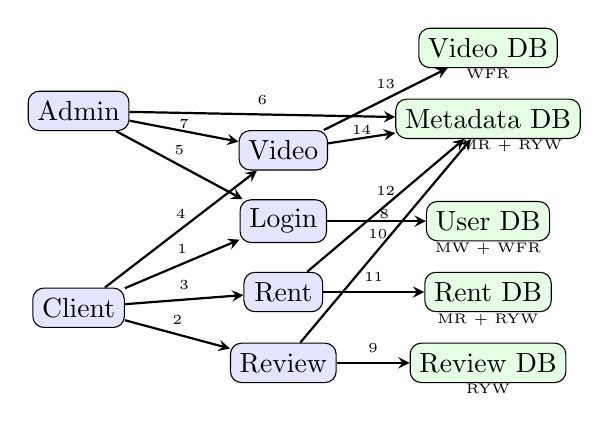
\begin{tikzpicture}[
      node distance=1.8cm,
      service/.style={draw, rounded corners, fill=blue!10, minimum
      width=1cm, minimum height=0.5cm},
      storage/.style={draw, rounded corners, fill=green!10, minimum
      width=1cm, minimum height=0.5cm},
      arrow/.style={->, >=stealth, thick},
      label/.style={font=\small\itshape}
    ]
    % client and admin
    \node[service] (client) at (0,0) {Client};
    \node[service, yshift=3mm] (admin) at (0,2.2) {Admin};

    % services
    \node[service] (login) at (2.6,1.1) {Login};
    \node[service] (review) at (2.6,-0.7) {Review};
    \node[service] (rent) at (2.6,0.2) {Rent};
    \node[service] (video) at (2.6,2.0) {Video};

    % db nodes
    \node[storage] (user_db) at (5.2,1.1) {User DB};
    \node[storage] (metadata_db) at (5.2,2.4) {Metadata DB};
    \node[storage] (review_db) at (5.2,-0.7) {Review DB};
    \node[storage] (rent_db) at (5.2,0.2) {Rent DB};
    \node[storage] (video_db) at (5.2,3.3) {Video DB};

    % edges from client with centered, above labels
    \draw[arrow] (client) -- (login) node[pos=0.5, above, font=\tiny] {1};
    \draw[arrow] (client) -- (review) node[pos=0.5, above, font=\tiny] {2};
    \draw[arrow] (client) -- (rent) node[pos=0.5, above, font=\tiny] {3};
    \draw[arrow] (client) -- (video) node[pos=0.5, above, font=\tiny] {4};

    % edges from admin
    \draw[arrow] (admin) -- (login) node[pos=0.5, above, font=\tiny] {5};
    \draw[arrow] (admin) -- (metadata_db) node[pos=0.5, above, font=\tiny] {6};
    \draw[arrow] (admin) -- (video) node[pos=0.5, above, yshift=-1mm,
    font=\tiny] {7};

    % service to DB edges
    \draw[arrow] (login) -- (user_db) node[pos=0.5, above,
    xshift=1mm, yshift=-1mm, font=\tiny] {8};
    \draw[arrow] (review) -- (review_db) node[pos=0.5, above, font=\tiny] {9};
    \draw[arrow] (review) -- (metadata_db) node[pos=0.5, above,
    xshift=-1mm, yshift=-1mm, font=\tiny] {10};
    \draw[arrow] (rent) -- (rent_db) node[pos=0.5, above, font=\tiny] {11};
    \draw[arrow] (rent) -- (metadata_db) node[pos=0.5, above, font=\tiny] {12};
    \draw[arrow] (video) -- (video_db) node[pos=0.5, above, font=\tiny] {13};
    \draw[arrow] (video) -- (metadata_db) node[pos=0.5, above,
    yshift=-0.8mm, font=\tiny] {14};

    % semantics for databases only
    \node[below=0.15cm, align=center, font=\tiny] at (user_db) {MW + WFR};
    \node[below=0.15cm, align=center, xshift=3mm, font=\tiny] at
    (metadata_db) {MR + RYW};
    \node[below=0.15cm, align=center, font=\tiny] at (review_db) {RYW};
    \node[below=0.15cm, align=center, font=\tiny] at (rent_db) {MR + RYW};
    \node[below=0.15cm, align=center, font=\tiny] at (video_db) {WFR};
  \end{tikzpicture}
  \caption{Architecture of the media streaming service with
    consistency guarantees.
    Edges are numbered for reference:
    1–4: Client requests to services (login, review, rent, video).
    5: Admin login.
    6: Admin updates metadata.
    7: Admin uploads video.
    8: Login service accesses User DB.
    9: Review service writes to Review DB.
    10: Review checks content existence in Metadata DB.
    11: Rent updates Rent DB.
    12: Rent checks content availability in Metadata DB.
    13: Video service accesses Video DB.
  14: Video service verifies metadata before playback.}
  \label{fig:case-study-media}
\end{figure}

\begin{enumerate}[noitemsep,topsep=2pt,left=5pt]
  \item \textbf{Client and Admin}: These components represent the
    entry points for regular users and administrative personnel,
    respectively. They don't enforce specific consistency guarantees
    themselves but rely on the guarantees provided by the services
    they interact with.

  \item \textbf{Authentication}:
    \begin{itemize}[noitemsep,topsep=0pt,left=5pt]
      \item \textbf{Login Service}: Manages user authentication and
        session handling. It requires order preserving writes
	for correct credential update and user's updates 
	(e.g., subscription status change) must be always visible for
	flawless service.
      \item \textbf{User DB}: A \sysmod{} that stores user credentials and
        profile information. MW and WFR ensures
        that when users update their profiles or credentials, these
        changes are consistently visible to subsequent operations.
    \end{itemize}

  \item \textbf{Content Management}:
    \begin{itemize}
      \item \textbf{Metadata Database}: Stores information about
        available media content (titles, descriptions, genres, etc.)
        with Monotonic Reads (MR) and Read Your Writes (RYW)
        guarantees. This allows administrative updates to be
        immediately visible while tolerating some staleness for user reads.
      \item \textbf{Video Service}: Handles video streaming requests
        and requires MR guarantees to ensure consistent content delivery.
      \item \textbf{Video Database}: Stores the actual video content
        with WFR guarantees to maintain version consistency.
    \end{itemize}

  \item \textbf{API}:
    \begin{itemize}
      \item \textbf{Review Service}: Manages user reviews and
        requires RYW guarantees to ensure users can immediately see
        their own reviews.
      \item \textbf{Review Database}: Stores user reviews with RYW
        guarantees, allowing users to see their own reviews
        immediately while other users might see slightly stale data.
      \item \textbf{Rent Service}: Handles media rental transactions
        and requires MR guarantees to ensure consistent inventory checks.
      \item \textbf{Rent Database}: Records rental transactions with
        MR and RYW guarantees to maintain consistent transaction history.
    \end{itemize}
\end{enumerate}

{\color{red}
  In this example, we've specified that all users must register for
  an account before they can log in, this would result in a request from
  client to login service (edge 1), then to user database (edge 8).
  If users are to post a review (edge 2), they must
  be logged in (edge 1), and the review service must verify that the
  title exists
  in the metadata database (edge 10) before allowing the review to be
  written (edge 9).
  This is one of the clear dependency chains in the media service example.
  This dependency chain creates a cascading effect throughout the system
  where each operation builds upon the successful completion of its
  prerequisites.
  The registration-before-login dependency establishes user identity,
  the login-before-content-access dependency establishes authorization,
  and the content-validation-before-review dependency establishes
  referential integrity.

  Semantically, 6 nodes are interacting with each other (client,
    login service, user database, review service, metadata database,
  and review database) in the aforementioned dependency chain.
  The edges between these nodes represent the flow of API requests and we
  encode the prerequisites of each request as constraints on edges.
  Implementation-wise, all constraints on edges can be
  directly encoded on the nodes themselves along with our
  predefined semantics. However, when modeling
  services with complex interactions with cross storage system
  dependencies, edge constraints can clearly
  separate the providing/requiring semantic constraints and
  downstream implementation specific
  service logic. In the implementation, we defined multiple operations
  with read or write type to represent interactions between client,
  service nodes, and storage nodes.
  Formally, we can represent client's login operation as follow:

  \begin{align*}
    EC_{login} &\triangleq \forall op_{login} \in H_{rd} : \exists
    op_{reg} \in H_{wr} :\\
  &ob(op_{login}, op_{reg}) \land vis(op_{reg}, op_{login}))
\end{align*}

For services initiated from the client side, we modeled the behaviors
as a set of re-useable common constraints with the return-before
binary relationship. Formally:

\begin{align*}
  EC_{auth} &\triangleq rb(op_{login}, op_{rdreview}) \land
  rb(op_{login}, op_{wrreview}) \\
  &\land rb(op_{login}, op_{rent}) \land rb(op_{login}, op_{watch})
\end{align*}

The common constraints are then added to each edge that's dependent on the
login service or refer to the login operation, ensuring the chain
of dependencies is respected throughout the system. For posting reviews,
the review service must first verify that the content exists in the
metadata database before allowing the review to be written. Similar to
the login operation, we can represent the review service's interaction
as a set of constraints with existential quantification, object constraints,
and return-before relationships, on top of consistency semantics
encoded at each nodes' provide and need fields.

\begin{align*}
  EC_{review} &\triangleq \forall op_{review} \in H_{wr} : \exists
  op_{rdmeta} \in H_{rd} :\\
  &ob(op_{review}, op_{rdmeta}) \land rb(op_{rdmeta}, op_{review})
\end{align*}
}

\subsubsection{Interaction Flows}

The media streaming service supports several interaction patterns,
each with specific consistency requirements:

\textbf{User Registration and Authentication}: Before accessing any
content, users must register and authenticate through the login
service. This process involves:

\begin{enumerate}
\item The client sends a registration request (abstracted as a
  write operation) to the login service.
\item The login service writes the new user credentials to the User Database.
\item For subsequent logins, the client sends a login request
  (abstracted as a read operation) to the login service.
\item The login service reads from the User Database to verify credentials.
\end{enumerate}

The MW and WFR guarantees of the User Database ensure that once user
credentials are updated, all subsequent authentication attempts will
see the updated information, preventing authentication anomalies
where users might be unable to log in with newly created or changed credentials.

\textbf{Browsing and Playback}: Once authenticated, users can browse
and watch available content:

\begin{enumerate}
\item The client sends a request to browse content, which queries
  the Metadata Database.
\item When a user selects content to watch, the client sends a
  request to the Video Service.
\item The Video Service verifies the content's existence and
  availability by reading from the Metadata Database.
\item If the content is available, the Video Service streams the
  content from the Video Database to the client.
\end{enumerate}

The MR guarantee of the Video Service ensures that once a piece of
content is determined to be available, subsequent read operations
will maintain this view, preventing inconsistencies during playback.
The WFR guarantee of the Video Database ensures that if the service
reads a specific version of content, subsequent writes will not
revert to an earlier version.

\textbf{Rentals}: For premium content, users must first rent the content:

\begin{enumerate}
\item The client sends a rental request to the Rent Service.
\item The Rent Service checks content availability by reading from
  the Metadata Database.
\item If available, the Rent Service records the transaction in the
  Rent Database.
\item The client can then access the rented content through the Video Service.
\end{enumerate}

The MR guarantee of the Rent Service ensures consistent inventory
checks, preventing scenarios where content appears to be available
and then becomes unavailable during the rental process.

\textbf{Reviews}: Users can read and write reviews for content they've watched:

\begin{enumerate}
\item To read reviews, the client sends a request to the Review
  Service, which retrieves reviews from the Review Database.
\item To write a review, the client sends the review content to the
  Review Service.
\item The Review Service verifies that the content exists by
  reading from the Metadata Database.
\item If verified, the Review Service writes the review to the
  Review Database.
\end{enumerate}

The RYW guarantee of both the Review Service and Review Database
ensures that users immediately see their own reviews after
submission, providing a responsive user experience while allowing for
eventual consistency for other users' views.

\textbf{Admin Operations}: Administrators manage content through
separate workflows:

\begin{enumerate}
\item Administrators authenticate through the Login Service (with
  pre-granted access).
\item To add new content, administrators:
  \begin{itemize}
    \item Upload video content to the Video Database through the
      Video Service.
    \item Add corresponding metadata to the Metadata Database.
  \end{itemize}
\item To modify user accounts, administrators interact with the
  Login Service, which updates the User Database.
\end{enumerate}

The combination of RYW and MR guarantees in the Metadata Database
ensures that administrative updates are immediately visible to the
administrators themselves while allowing for controlled propagation
to user-facing services.

\subsubsection{Requirements and Verification}

Each component in the system has specific consistency requirements
based on its functional role:

\begin{itemize}
\item The User Database provides MW and WFR guarantees, ensuring
  that credential updates are properly sequenced and visible, which
  is critical for authentication security.

\item The Metadata Database provides MR and RYW guarantees,
  balancing immediate visibility of administrative updates with
  tolerance for some staleness in user reads.

\item The Review Database provides RYW guarantees, prioritizing the
  user experience of seeing one's own reviews immediately while
  accepting eventual consistency for other users' views.

\item The Rent Database provides MR and RYW guarantees, ensuring
  consistent transaction records for both administrative and user views.

\item The Video Database provides WFR guarantees, maintaining
  version consistency for content delivery.
\end{itemize}

The edges in our model represent not just data flow but also critical
operational constraints. For example, the edge from the Client to the
Login Service carries the constraint that "User must register before
login," enforced through a visibility relationship between
registration and login operations. Similarly, the edge from the
Review Service to the Metadata Database enforces the constraint that
"Check metadata before read review," ensuring that reviews are only
accessible for valid content.

When we apply \texttt{composable} function to this system,
starting from the client node, it successfully verifies that the
composition of these services with their respective consistency
guarantees satisfies the overall system requirements. The function
traverses the graph, checking at each step whether the constraints
imposed by each node and edge are mutually satisfiable.

This verification confirms that despite the heterogeneous consistency
guarantees across different components, the system as a whole
maintains its required properties. For instance, the login flow
correctly enforces that registration must precede login, and the
review system correctly ensures that users can immediately see their
own reviews while maintaining content validity checks.



